
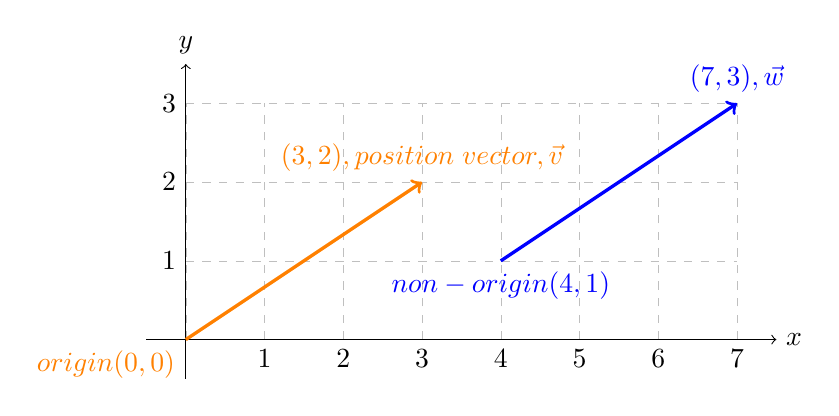
\begin{tikzpicture}
    \draw[step=1,help lines, dashed,lightgray] (0,0) grid (7,3);
    %draw axis value
    \foreach \x in {1,2,3,4,5,6,7}
        {%
            \draw (\x,0) -- (\x,0) node [below] {$\x$};
        }
    \foreach \y in {1,2,3}
        {%
            \draw (0,\y) -- (0,\y) node [left] {$\y$};
        }
    %draw lines
    \draw [->] (-0.5,0) -- (7.5,0) node[right]{$x$};
    \draw [->] (0,-0.5) -- (0,3.5) node[above]{$y$};
    \draw [->,orange,very thick] node[below left]{$origin (0,0)$} (0,0) -- (3,2) node[above]{$(3,2), position\hspace{1mm}vector, \vec{v}$};
    \draw [->,blue,very thick]  (4,1) node[below]{$non-origin (4,1)$} -- (7,3) node[above]{$(7,3), \vec{w}$};
\end{tikzpicture}
\captionof{figure}{{\footnotesize $\vec{w}$ ပုံစံကနေ $\vec{v}$ သို့ ပြောင်းလဲခြင်း}}
\label{fig:vector-and-vector-operation-d5}
